\documentclass[twoside,11pt]{article}

\usepackage{blindtext}

% Any additional packages needed should be included after jmlr2e.
% Note that jmlr2e.sty includes epsfig, amssymb, natbib and graphicx,
% and defines many common macros, such as 'proof' and 'example'.
%
% It also sets the bibliographystyle to plainnat; for more information on
% natbib citation styles, see the natbib documentation, a copy of which
% is archived at http://www.jmlr.org/format/natbib.pdf

% Available options for package jmlr2e are:
%
%   - abbrvbib : use abbrvnat for the bibliography style
%   - nohyperref : do not load the hyperref package
%   - preprint : remove JMLR specific information from the template,
%         useful for example for posting to preprint servers.
%
% Example of using the package with custom options:
%
% \usepackage[abbrvbib, preprint]{jmlr2e}

\usepackage{amsmath}
\usepackage[preprint]{jmlr2e}

% Definitions of handy macros can go here

\newcommand{\dataset}{{\cal D}}
\newcommand{\fracpartial}[2]{\frac{\partial #1}{\partial  #2}}

% Heading arguments are {volume}{year}{pages}{date submitted}{date published}{paper id}{author-full-names}

\usepackage{lastpage}
\jmlrheading{23}{2025}{1-\pageref{LastPage}}{1/21; Revised 5/22}{9/22}{21-0000}{Yaoshiang Ho}

% Short headings should be running head and authors last names

\ShortHeadings{Supervised Learning Preference Optimization}{Yaoshiang Ho}
\firstpageno{1}

\begin{document}

\title{Supervised Learning Preference Optimization: Rethinking RLHF and DPO as Supervised Learning}

\author{\name Yaoshiang Ho \email yaoshiang@gmail.com \\
      %  \addr Department of Statistics\\
      %  University of Washington\\
      %  Seattle, WA 98195-4322, USA
      %  \AND
      %  \name Author Two \email two@cs.berkeley.edu \\
      %  \addr Division of Computer Science\\
      %  University of California\\
      %  Berkeley, CA 94720-1776, USA
      }

\editor{}

\maketitle 

\begin{abstract}%   <- trailing '%' for backward compatibility of .sty file
Direct Policy Optimization (DPO) is a popular approach to aligning 
large language models with human preferences. 
In this paper, we analyze the underlying math and 
propose a new algorithm
which we call Supervised Learning Preference Optimization (SLPO). 
 
\end{abstract}

\begin{keywords}
  Reinforcement Learning from Human Feedback (RLHF), Direct Policy Optimization (DPO)
\end{keywords}

\section{Introduction}

Alignment is the task of ensuring that the behavior of a
Large Language Model (LLM) is consistent 
with human preferences. 

A key difference between the alignment phase and
other phases of training an LLM is that the alignment phase considers
full sequences of text, rather than simply predicting the next token, as
in the pretraining and supervised fine-tuning (SFT) phases. 

The alignment approach popularized by the commercial success of ChatGPT was 
Reinforcement Learning from Human Feedback (RLHF, \cite{ouyang2022training}). 
Despite its effectiveness, RLHF requires training a second model, called
a reward model, as well as Proximal Policy Optimization (PPO), resulting in a 
technique that is more complex than the basic supervised learning. It also
requires a Kullback-Leibler (KL) divergence term to regularize the
changes to the LLM during alignment training.

Direct Policy Optimization (DPO) is a simpler approach to alignment
which does not require a secondary reward model. In the paper introducing
DPO, the authors examine the underlying
approach of RLHF and propose
the DPO objective to align the target LLM directly using
maximum likelihood estimation (MLE). 
The key insight from the DPO paper is that an LLM's
outputs can be reparameterized into a reward model using ratios, logs,
and the Bradley-Terry model (\cite{bradley1952rank}).

The specific contribution of this paper is to reframe the alignment
phase away from reward modeling entirely and treating it simply as
a pure supervised learning problem by training a model to align to
a directly modified probability distribution. We call this
approach Supervised Learning Preference Optimization (SLPO).

\section{Related Work}

Related work\dots

\section{Preliminaries: DPO}

We review and continue the analysis of the DPO objective by its 
authors.

The DPO objective is defined as follows:

\begin{equation}
  \label{eq:dpo}
  L_\mathrm{DPO}(\pi_\theta; \pi_\mathrm{ref}) =
  \underbrace{
  -\mathbb{E}_{(x, y_w, y_l) \sim D} 
  \log }_{1} 
  \left[ 
    \underbrace{\sigma }_{2}
    \left(
    \underbrace{\beta \log \frac{\pi_\theta(y_w \mid x)}{\pi_\mathrm{ref}(y_w \mid x)}}_{3}
    - \underbrace{\beta \log \frac{\pi_\theta(y_l \mid x)}{\pi_\mathrm{ref}(y_l \mid x)}}_{4} 
    \right)
  \right].
\end{equation}

In the underbraced section 1, we see the standard 
negative log likelihood (NLL) objective.
In the underbraced section 2, we see the Bradley-Terry model 
\footnote{A ranking method that is mathematically equivalent and perhaps more 
widely understood is the ELO score, used to rank Chess players, 
and, LLMs in the Chatbot Arena (\cite{elo1978rating,chiang2024chatbot}). 
Both ELO and Bradley-Terry assign scores to players, and 
pass the difference through a sigmoid function to assess the probability of 
the LHS player of winning. }.
In the underbraced sections 3 and 4, we see how the 
reference and language model's predictions are reparameterized
into a winning and losing score: they are the 
log of the ratio of the language model to the reference model, for the winning and 
losing completion, respectively. 
This score is later described as the reward function.

With simple algebraic manipulation, we can rewrite this objective as:

\[
  \label{eq:reg}
  L_\mathrm{DPO}(\pi_\theta; \pi_\mathrm{ref}) =
  \underbrace{
  -\mathbb{E}_{(x, y_w, y_l) \sim D} 
  \log }_{1} 
  \left[ 
    \underbrace{\sigma }_{2}
    \left(
    \underbrace{\beta \log \frac{\pi_\theta(y_w \mid x)}{\pi_\theta(y_l \mid x)}}_{3}
    - \underbrace{\beta \log \frac{\pi_\mathrm{ref}(y_w \mid x)}{\pi_\mathrm{ref}(y_l \mid x)}}_{4} 
    \right)
  \right].
\]

We can interpret the undercomponents as follows: 
The first and second underbraces remain unchanged. 
The third underbrace is the log of the ratio
language models probability of the winner divided by the loser. This ratio 
is optimized to be bigger, given that the log, sigmoid, and log from underbraces
1, 2, and 3 are all monotonic functions. Since a ratio of probabilities is
an odds ratio, we will refer to this as the 
language model's log-odds ratio. 

The fourth underbrace is reference model's log-odds ratio. This
is a constant per $y_w$ and $y_l$ and is not differentiated. However,
these values and their ratio vary across different $y_w$ and $y_l$ - that is,
each row of training data will have a different value for this constant. 
More specifically, since $\pi_\theta$ is initialized as $\pi_\mathrm{ref}$, 
the difference between underbraces 3 and 4 starts at zero during training, 
and the shape of the sigmoid function (underbrace 2) and its gradient are
known. During training, as the language model's log-odds ratio increases,
the sigmoid function will naturally regularize and decelerate
the increase by reducing the magnitude of the gradient (a 
useful version of the vanishing gradient problem). 
This is the exact outcome described by the DPO authors 
in their analysis of the gradient of DPO. \emph{But we have developed a different
intuition the DPO loss: rather than reparameterizing the language model's
output into a reward model, we are simply regularizing the optimization of 
the language model's log-odds ratio.}

Let's analyze the regularization effect. The DPO authors investigated
the gradient of the sequence of tokens... let's go two steps further
by considering each token individually, and the softmax logit behind it \footnote{
  Technically, a logit is the log-odds ratio and it is the output of a 
  feature extractor before a sigmoid activation function in binary
  classification. The term logit is also used for categorical classification,
  when a feature extractor's outputs are 
  activated with the softmax function. However,
  these softmax logits cannot be expontentiated to calculate an odds ratio. 
  They do have an unfortunately property
  however: they are shift invariant, leading to numerical instability and
  the need for log-softmax and its use of the log-sum-exp trick to improve
  numerical stability. In this paper, since we are dealing
  with both sigmoid and softmax functions, we will refer to the value
  passed into a softmax function as a softmax logit.
}. 

The variable $y$ is a sequence of tokens, defined as

\begin{equation}
  \label{eq:joint}
  \pi_\mathrm{ref}(y \mid x) = \prod_{t=1}^T \pi_\mathrm{ref}(y_t \mid x, y_{<t}),
\end{equation}

where \(y = (y_1, y_2, \ldots, y_T)\) is the output sequence, 
\(x\) is the input context, and \(y_{<t} = (y_1, y_2, \ldots, y_{t-1})\) 
represents the tokens generated prior to time step \(t\). The term 
\(\pi_\mathrm{ref}(y_t \mid x, y_{<t})\) denotes the conditional 
probability of generating token \(y_t\) given the input \(x\) and 
the previously generated tokens \(y_{<t}\).

Since both $\pi$ language model are LLMs, they are activated
using the softmax function. 
The softmax operation can be mathematically cumbersome 
due to its dependence on all other logits for normalization. 
For simplicity, we assume that the logits are transformed 
using a log-softmax function, which computes the logarithm 
of the softmax probabilities in a numerically stable way. 
This transformation results in log-probs, 
which are easier to reason about since they 
can be exponentiated to recover probabilities. 
Importantly, we do not lose any generality because 
log-probs can also be passed through a softmax 
function to recover probabilities, ensuring equivalent behavior.

Let us establish the term $\mathrm{g}$ for the layers of the model up to the softmax
activation, namely, the feature extractor and log-softmax normalization: 

\begin{equation}
  \label{eq:g}
  \mathrm{g}(y \mid x) = \mathrm{logsoftmax}(\mathrm{f}(y \mid x))
\end{equation}
such that
$
  \pi(y \mid x) = \exp (\mathrm{g}(y \mid x)).
$
Plugging Equations ~\ref{eq:joint} and ~\ref{eq:g} into the DPO objective ~\ref{eq:dpo}, 
\begin{multline}
  \nonumber
  L_\mathrm{DPO}(\pi_\theta; \pi_\mathrm{ref}) = 
  -\mathbb{E}_{(x, y_w, y_l) \sim D} 
  \log \\ 
  \left[
    \sigma 
    \left(
      \beta \log \frac
      {\prod_{t=1}^{T_w} \exp (\mathrm{g_\theta}(y_{w,t} \mid x, y_w{<t}))}
      {\prod_{t=1}^{T_w} \exp (\mathrm{g_\mathrm{ref}}(y_{w,t} \mid x, y_w{<t}))}
      - 
      \beta \log \frac
      {\prod_{t=1}^{T_l} \exp (\mathrm{g_\theta}(y_{l,t} \mid x, y_w{<t}))}
      {\prod_{t=1}^{T_l} \exp (\mathrm{g_\mathrm{ref}}(y_{l,t} \mid x, y_w{<t}))}
      \right)
      \right]
    \end{multline} 
which simplifies to: 
\begin{multline}
  L_\mathrm{DPO}(\pi_\theta; \pi_\mathrm{ref}) = 
  -\mathbb{E}_{(x, y_w, y_l) \sim D} 
  \log \\ 
  \left[
    \sigma 
    \left(
      \beta 
        \left( 
          \sum_{t=1}^{T_w} \left[ \mathrm{g_\theta}(y_{w,t} \mid x, y_{w,<t}) - \mathrm{g_\mathrm{ref}}(y_{w,t} \mid x, y_{w,<t}) \right] 
          - 
          \sum_{t=1}^{T_l} \left[ \mathrm{g_\theta}(y_{l,t} \mid x, y_{l,<t}) - \mathrm{g_\mathrm{ref}}(y_{l,t} \mid x, y_{l,<t}) \right] 
        \right)
    \right)
  \right]
\end{multline}

We notice another possibility to rewrite the DPO objective towards something
more familiar. Optimizing the sigmoid of a difference $a-b$ through BCE 
is equivalent to optimizing the softmax of $a$ and $b$ through CCE towards 
a one-hot encoded target of softmax(a) = 1 and softmax(b) = 2. This allows
us to rewrite the DPO objective as follows:

\begin{equation}
\label{eq:dpo-as-cce}
L_\mathrm{DPO}(\pi_\theta; \pi_\mathrm{ref}) = 
-\mathbb{E}_{(x, y_w, y_l) \sim D} \, 
\text{CCE}
\left[
y_\mathrm{true} = 
\begin{bmatrix}
1 \\ 
0
\end{bmatrix}
\right]
,
y_\mathrm{pred} = \text{softmax}
\left(
\begin{bmatrix}
\beta S_w \\ 
\beta S_l
\end{bmatrix}
\right)
\end{equation}
where
\[S_w = \sum_{t=1}^{T_w} \big(\mathrm{g_\theta}(y_{w,t} \mid x, y_{w,<t}) - \mathrm{g_\mathrm{ref}}(y_{w,t} \mid x, y_{w,<t})\big),
\]
\[
S_l = \sum_{t=1}^{T_l} \big(\mathrm{g_\theta}(y_{l,t} \mid x, y_{l,<t}) - \mathrm{g_\mathrm{ref}}(y_{l,t} \mid x, y_{l,<t})\big).
\]

\paragraph{Key Observation \#1: Much of the DPO objective 
can be simplified to the form of a 
standard classification task.} \label{obs:dpo-as-cce}
This formulation of the DPO objective provides our first key observation. 
What started off as a complex reparameterization 
of the language model's output into a reward
model and a Bradley-Terry model, 
has been simplified into a standard 
categorical crossentropy loss applied to the softmax, in
Equation~\ref{eq:dpo-as-cce}. However, the
input to the softmax is not a single value, 
it's a sum of differences of values. That difference, and that
sum, are the remaining nuances to resolve. 

\paragraph{Key Observation \#2: The ratio of probabilities
creating a reward reward function has been transformed into a normalization of 
logits to make equivalent all the gradients at the start of training.} 

The first remaining nuance is the difference between
the language model and the reference model's logits. Since
the language model is initialized by the reference model,
the difference starts at zero for both $S_w$ and $S_l$. 
This means that at the start of training, all the gradients
for all the winning sequences examples will be the same as each other
(likewise for the losing sequences). 

\paragraph{Key Observation \#3: blah.} 
\label{obs:softmax-cce}
The second remaining nuance is that the softmax is applied to
the sum of the inputs, where the inputs were originally
softmax logits during the CCE(softmax()) applied during next
token prediction pretraining. 

What happens when we the input to a softmax is a sum? This is 
easy to reason about. At first, the gradient to each $S_w$ will
be 0.5, and that gradient will be passed through to each
value $z_t$. In turn, as $z_t$ is updated by a gradient, the collective
value of $S_w$ will increase far more than the value of $z_t$. 
In fact, during the first step, the update will be roughly
$T \times$ greater than the update to $z_t$, ignoring the effects 
of adaptive optimizers. So the value of $y_\mathrm{w}$ will increase
quickly... and in doing so, rapidly approach the 

is updated du, the collective update to
$S_w$ will increase far more than the value of $z_t$. In fact,
the update will approximate , and the gradient will decrease. This is 

=
XXX

XXX

XXX

XXX

XXX

XXX


The "logit" to the 
Each softmax logit of the language model, which was originally conceived to predict the probability of a token,
has been normalized by the softmax logit of the reference model via a shift (this normalization
should not to be confused with the normalization
by the log-softmax function, which was purely for mathematical convenience). The 
sum of these normalized softmax logits is then passed through a standard sigmoid activation and 
negative log likelihood function.

The starting value for the difference between the language model 
and the reference model's logits is zero, since the language model is initialized
by the reference model, so the gradient passed to each logit on the first step of 
optimization is -0.5 for the winning token and 0.5 for the losing token. As the 
winning sequence increases its odds, and the losing sequence decreases its odds,
the gradient will decrease, as is well known for the negative log loss applied
to a sigmoid activated function (e.g. classic binary crossentropy loss for
logistic regression). Although sigmoid is not an additive function, 
e.g. $\sigma(a + b) \neq \sigma(a) + \sigma(b)$, it is monotonically increasing,
e.g. $\sigma(a + b) > \sigma(a)$ where $b > 0$. So as the softmax logit of
each winning token increases and each losing token decreases, the magnitude of the
gradient applied to all softmax logits decreases.

And yet, the DPO equation involves significant 
machinery—such as the Bradley-Terry model, 
the log of ratios, and the concept of 
reward functions—
for what ultimately reduces to a standard 
negative log-likelihood loss applied to 
normalized softmax logits. Could this normalization 
be further simplified, perhaps eliminating 
the need for these additional constructs and 
reframing the problem in a more straightforward way?

\section{Preliminaries: Probabilistic Classification}

A basic task for deep learning has been classification, both
binary and categorical. Which of the ten digits is this image(\cite{lecun1998mnist})?
Is this pixel
part of an object's mask? Is this movie review's sentiment positive or
negative(\cite{Pang+Lee:04a})? 

Modern LLMs auto-regressively predict a probability distribution for 
the next token among a finite set of possibilities, conditioned on the 
previous tokens. Hence, an LLM also solves 
a classification problem. 

Given the prevalence of classification, deep learning oftens assumes
target labels can be described as either ordinal numbers
or equivalently one-hot encoded vectors. When target labels are
intermediate values between one and zero, they were called "soft targets", 
treated as an regularization technique or even called dark knowledge
(\cite{hinton2015distilling, szegedy2016rethinking,hinton2014dark}). 

But the two roots of the crossentropy
loss functions: KL divergence and Maximum Likelihood Estimation (MLE) applied
to the probability distribution function of a Multi-Bournoulli
distribution, are not limited to binary and categorical outcomes. 
For example, the crossentropy loss function can be used directly 
to condition a model to predict to be true 60\% of the time and false 40\% of 
the time, as demonstrated in Figure \ref{fig:ce06}. 
\begin{figure}[htbp]
  \centering
  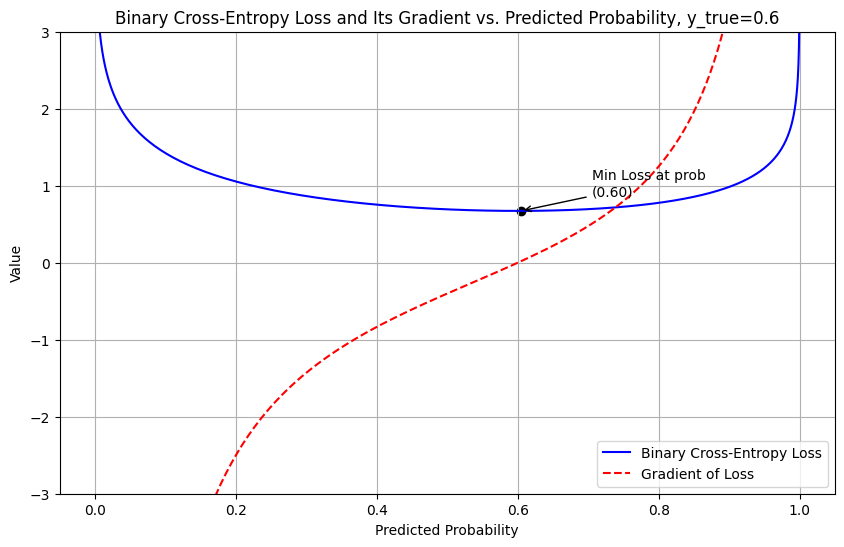
\includegraphics[width=0.8\textwidth]{ce06.png}
  \label{fig:ce06}
  \caption{Setting $y_\mathrm{true}$ to a value 
  other than 0 or 1 is a valid 
  use of the crossentropy loss 
  function and perfectly consistent with
  both KL divergence and MLE.}
\end{figure}

The term we will use for the idea of
predicting a probability distribution is \emph{probabilistic classification}.

\section{Supervised Learning Preference Optimization}

Armed with intuition of the DPO loss and probabilistic classification, we can
now turn to a simpler, supervised learning approach to alignment.

The SLPO objective is defined as follows:

\[
  L_\mathrm{SLPO}(\pi_\theta; \pi_\mathrm{ref}) =
  -\mathbb{E}_{(x, y_w, y_l) \sim D} 
\]
\[
  \left(
  \log\big(
    \underbrace{
      w_w * \pi_\theta(y_w \mid x)
    }_{1}
  )
    + 
  \log\big(
    \underbrace{
      w_l * \pi_\theta(y_l \mid x)
    }_{2}
  )
  + 
  \log\big(
    \underbrace{
      (1 - w_w - w_l) * \pi_\theta(y_o \mid x)
    }_{3}
  ) 
  \right)
\]

where $w_w = \alpha * (\pi_\mathrm{ref}(y_w \mid x) + \pi_\mathrm{ref}(y_l \mid x)$),
$w_l = (1 - \alpha) * (\pi_\mathrm{ref}(y_w \mid x) + \pi_\mathrm{ref}(y_l \mid x)$). 


Intuitively, the goal is to take the probabilities of the winning
and losing sequence and reallocate them. If alpha is zero, then all of the
probability will be allocated to the winning sequence. Importantly,
the
sum of the probabilities of the winning and losing tokens will be the same in
the language model and the reference model. Obviously, this implies that 
the probability of all other sequences are optimized to be the same
in the language model and the reference model. 
This is essentially the SLPO's version of
the KL divergence regularization term in traditional RLHF. 

Note that there are no negative signs in the SLPO objective. This is because
the SLPO objective is a pure supervised learning objective, and the negative
sign in what the DPO paper calls the unlikelihood objective is not 
consistent with MLE, since MLE always applies the negative log loss to
probabilities, and probabilities are always positive. 

\section{Results}



% {\pi_\mathrm{ref}(y_w \mid x)}

% \frac{\pi_\theta(y_l \mid x)}

Section body

Here is a citation \cite{chow:68}.

\section{Conclusion}

Section body

Here is a citation \cite{chow:68}.

% Acknowledgements and Disclosure of Funding should go at the end, before appendices and references

\acks{The author thanks Chiara Cerini, Peter Tran, and Sam Wookey for their 
invaluable reviews of early drafts of this work.}

% Manual newpage inserted to improve layout of sample file - not
% needed in general before appendices/bibliography.

\newpage

\appendix
\section{}
\label{app:theorem}

% Note: in this sample, the section number is hard-coded in. Following
% proper LaTeX conventions, it should properly be coded as a reference:

%In this appendix we prove the following theorem from
%Section~\ref{sec:textree-generalization}:

[appendix]

\section{Equivalence of Cross-Entropy on Sigmoid of Difference
and Categorical Cross-Entropy on Softmax of True Class for Two Classes}

Logistic regression uses 
a single logit \(\alpha\), transforming it through the \emph{sigmoid} function to obtain 
a probability \(\sigma(\alpha) = \frac{1}{1 + e^{-\alpha}} \). The \emph{binary cross-entropy} 
(BCE) loss for a label $y$ and predicted probability \(\hat{y} = \sigma(\alpha)\) is:
\[
  \text{BCE}(y, \hat{y})
  \;=\;
  - \left[
      y \,\log(\hat{y})
      \;+\;
      (1 - y)\,\log (1 - \hat{y})
    \right].
\]

Alternatively, single-label multiclass classification of two 
outcomes uses two softmax logits \(z_1\) and \(z_2\) (one per class) 
and applies the softmax function to obtain probabilities:
\[
  p(y=1 \mid z_1, z_2)
  \;=\;
  \frac{e^{z_1}}{e^{z_1} + e^{z_2}},
  \qquad
  p(y=2 \mid z_1, z_2)
  \;=\;
  \frac{e^{z_2}}{e^{z_1} + e^{z_2}}.
\]
The associated categorical cross-entropy (CCE) loss is: 
\[
  \text{CCE}(y, \hat{y})
  \;=\;
  -\sum_{k=1}^2 y_k \,\log (\hat{y}_k ),
\]
where \(\hat{y}_1 = \frac{e^{z_1}}{e^{z_1} + e^{z_2}}\) and 
\(\hat{y}_2 = \frac{e^{z_2}}{e^{z_1} + e^{z_2}}\).

If we set 
\[
  \alpha = z_1 - z_2,
\]
then
\[
  \frac{e^{z_1}}{e^{z_1} + e^{z_2}}
  =
  \frac{1}{1 + e^{z_2 - z_1}}
  =
  \sigma(\alpha).
\]
Therefore, the predicted probability of class 1 in the softmax parameterization 
matches the \(\sigma(\alpha)\) in logistic regression. This means that 
the BCE loss on the sigmoid of a difference of two numbers ($z_1 - z_2$) 
is equivalent
to the CCE loss on the softmax of the first number
($z_1$) (\cite{Goodfellow-et-al-2016}).




{\noindent \em Remainder omitted in this sample. See http://www.jmlr.org/papers/ for full paper.}


\vskip 0.2in
\bibliography{sample}

\end{document}
